\documentclass[a4paper]{article}

\usepackage[utf8]{inputenc}
\usepackage{erk}
\usepackage{times}
\usepackage{graphicx}
\usepackage[top=22.5mm, bottom=22.5mm, left=22.5mm, right=22.5mm]{geometry}

\usepackage[slovene,english]{babel}
\usepackage{hyperref}
\usepackage{url}
\usepackage{float}

\let\oldfootnotesize\footnotesize
\renewcommand*{\footnotesize}{\oldfootnotesize\scriptsize}

\begin{document}
\title{Oddaja seminarske dokumentacije - 1. seminar pri predmetu Računalniška grafika in tehnologija iger}

\author{Aljaž Kozina, Denis Kotnik, Kristian Žarn, Klemen Červ}

\affiliation{	Univerza v Ljubljani, Fakulteta za računalništvo in informatiko }

\email{E-pošta: \\kozinc@gmail.com, \\
 denis.kotnik@gmail.com, \\kristian.zarn@gmail.com, \\klemen.cerv@gmail.com}

\maketitle

\selectlanguage{slovene}

\begin{abstract}{Povzetek}
V tretjeosebni pustolovščini vodimo ladjo, polno zaklada mimo nasprotnikov do pristanišča, medtem ko se trudimo, da bi izgubil čim manj zaklada.
\end{abstract}



\section{Pregled igre}
Naša igra je tretjeosebna pustolovščina, navdihnjena z igro Overboard!\cite{wiki:Overboard!}, v kateri igramo pirata, ki želi zbrati čimveč zaklada, brez da bi mu drugi pirati potopili ladjo. V zaprtem svetu se glavni igralec izogiba drugim ladjam ali pa jih napada s svojim orožjem medtem ko išče zaklad.

\begin{figure}[H]
    \begin{center}
        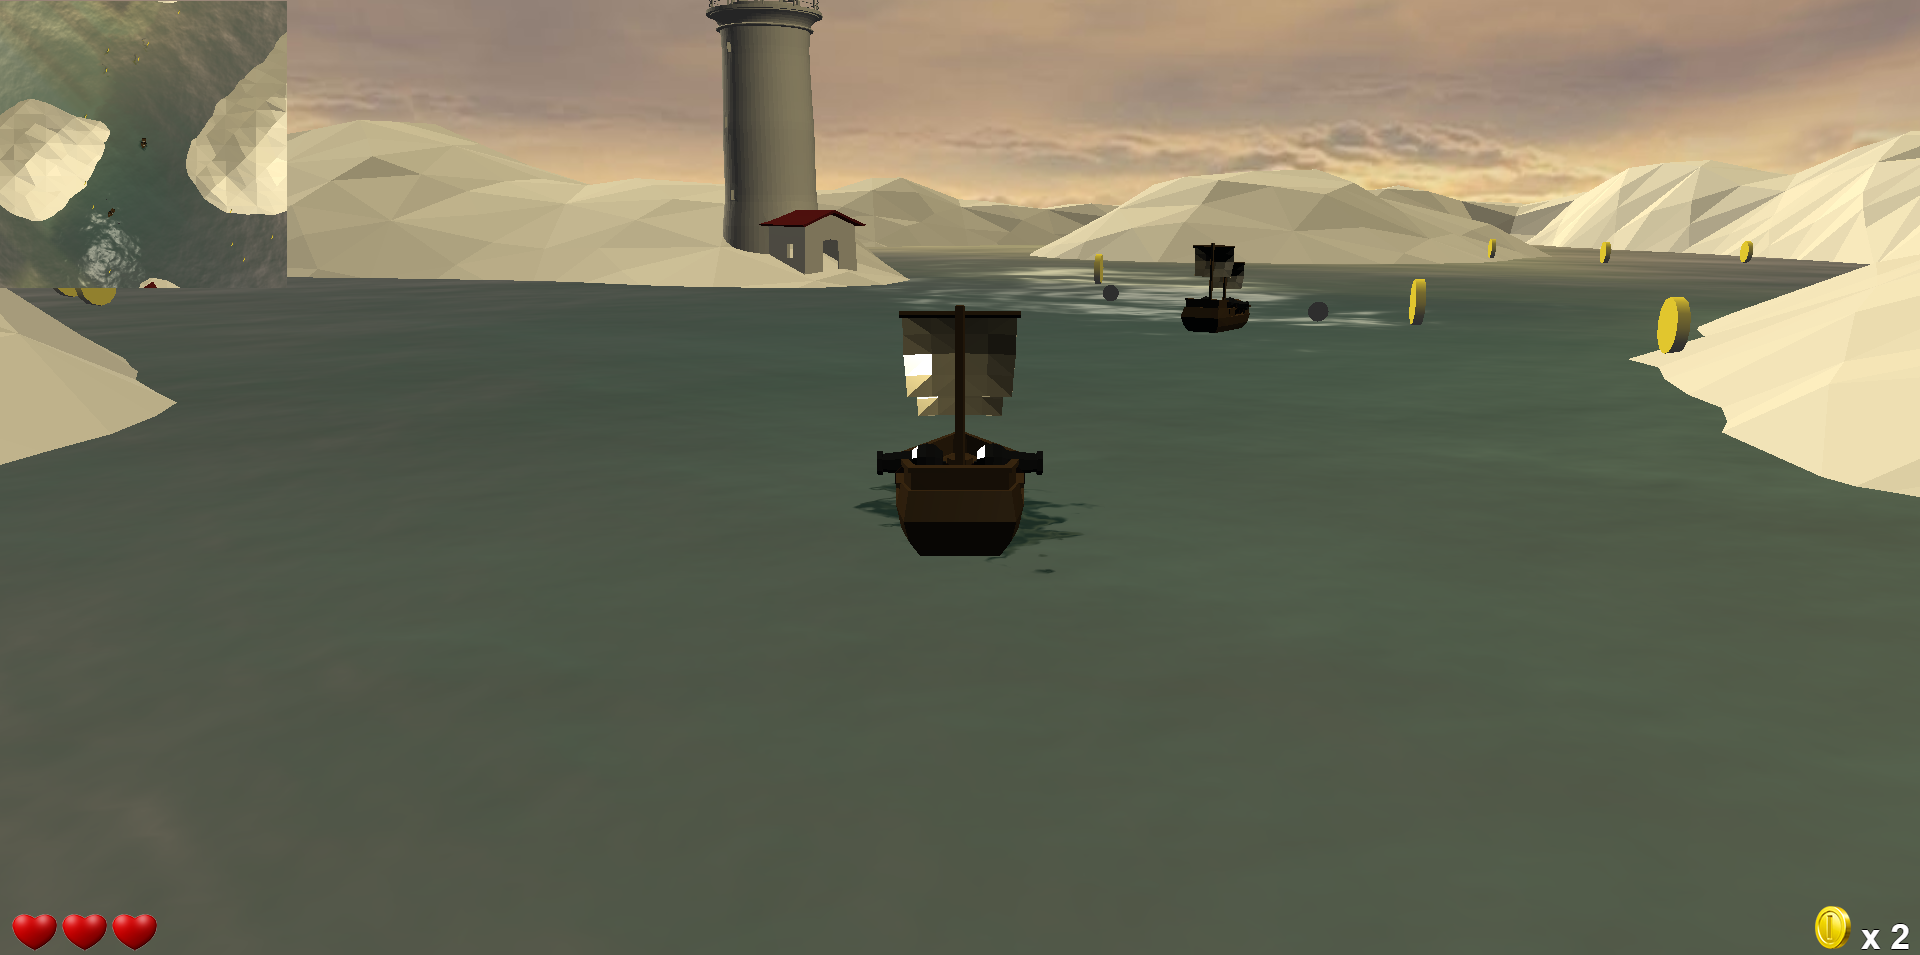
\includegraphics[width=\columnwidth]{Screenshot.png}
        \caption{Naša igra v WebGL.} \label{fig:slika}
    \end{center}
\end{figure}

\section{Seminarska dokumentacija}
\textit{Dokumentacija naj bo v formatu PDF in naj vsebuje do 5000 znakov. V dokumentaciji opišite delo v okviru seminarja. Opišite uporabljene pristope in metode, ki ste jih uporabili pri izdelavi seminarja. }

\subsection{Pregled}
Pri izdelavi našega seminarja smo uporabili tehnologije WebGL, Three.js\cite{wiki:Three.js}, itd. Za nalaganje 3D objektov smo uporabili OBJMTLLoader. Za prikaz vode smo uporabili shader, ki je vodi priredil animirano teksturo normal \href{http://github.com/jbouny/ocean}{z namenom prikaza realistične vode}.
Pri razvoju naše igre smo si pomagali z uporabo GitHuba. \\
\\
V trenutni različici igre, lahko igralec pobira cekine in strelja ladje. Njegov cilj je, da pobere čimveč cekinov, brez da bi ga nasprotniki potopili. Nasprotniki se gibajo po vnaprej določeni poti in streljajo, če igralec pride v bližino.


\subsection{Potek programa}
V naši igri se ob naložitvi okna inicializirajo potrebne spremenljive za igro, kot so scena, renderer, elementi HUD (življenje in rezultat) ter poslušalci tipkovnice. V sceni so ustvarjene tri kamere, dve za pogled igralca, tretja pa za prikaz mini-zemljevida z uporabo viewporta. \\
Nato se v sceno naložijo ladje - ladja igralca, pa tudi vsi sovražniki, ki se trenutno gibajo po prednastavljenih tirih. S pomočjo OBJMTL loaderja nato naložimo kopno, ki igralcu omejuje igralni prostor (vse ladje in kopno z uporabo metode addCollisionObject registriramo kot objekte, ki se jim preverja trčenje). Dodano je tudi pristanišče, ki pa kot igralni predmet trenutno še nima pomena. Nato je po zemljevidu naključno posejanih 50 kovancev, ki jih igralec s pomočjo metode checkCollect pobira in si tako povečuje rezultat. \\
V sceno so nato naloženi viri svetlobe (AmbientLight, 2x Directional Light), shaderji in pa Skybox, ki igralcu olepšajo svet.\\
Ko se igra naloži, se igralec nato lahko premika, strelja krogle (Krogla.js) in pobira kovance.

\subsection{Opis pomembnejših funkcij}

\begin{itemize}
\item \textit{updateHUD} - tukaj se posodobijo elementi HUD, trenutno življenje in kovanci
\item \textit{checkCollision} - tukaj preverimo trčenje med objekti
\item \textit{update} - tukaj posodabljamo premikanje objekta in zaznavamo trčenje (v primeru ladje, ob trčenju z kopnim ali drugo ladjo, premik in rotacijo izničimo)
\end{itemize}



\small
\bibliographystyle{ieeetr}
\bibliography{references}

\end{document}
